\section{Background \& Motivation}

In this section, we first provide the necessary background on 
distributed applications and the motivating example that we will
use throughout the paper. We then motivate the need for our
new consistency model and system.

\subsection{Distributed Applications}

A distributed application comprises two components: Users
interact with the application by sending messages to
\textit{application processes}, for instance, by submitting
an HTTP request. In response, the 
processes may perform local computation, exchange messages, or
interact with a back-end \textit{system}.

Such systems, such as databases or key-value stores, are typically
located within the same (or a nearby) data center as the application 
processes. They are designed to handle the challenges of
programming in distributed environments, such as fault-tolerance.

\subsection{Motivating Example: Photo-Sharing App}

Throughout the paper, we consider a simple but illustrative
example: a photo-sharing application. The application allows
users to upload and share their photos with other users.

In our example application, photos are organized into
albums. Both photos and albums are stored in a distributed,
linearizable~\cite{herlihy1990linearizability} key-value store
using a unique key. A photo's key maps to a binary blob, and
an album's key maps to structured data containing the keys of
all of its photos. If a key is read but is not present, the
key-value store returns \texttt{null}.

When a user uploads $N$ photos to an album, a Web server
issues $N+1$ operations: First, it inserts $N$ key-value
pairs, one for each photo. Second, it issues a read-modify-write
to append the new photos' keys to the album. To handle a request to
view an album, a Web server first reads the album's key and subsequently
reads (one at a time) each of its photo's binary blob before
returning the aggregated contents to the user.

% \wl{this example app is okay, but hopefully we can come up with a better one. This one isn't ideal because storing blob bodies in the data store is normal at small scale but unusual at large scale (where there are specific blob stores) and returning them in line is particularly unusual}
% \wl{ideally the example would not be based on existence of an object, which is easy for apps to fix with a retry loop}

\subsection{Consistency Models \& App Latency}

Programmers rely on a system's consistency model while building their applications. By defining the system's set of allowed behaviors, a consistency model permits programmers to ignore the system's implementation and instead focus on ensuring their applications are correct given these behaviors.

% \wl{It would be great to include an additional example of many system interactions beyond the Facebook paper, especially if it wasn't from a hyperscaler}
% Jeff: I managed to add another in Jeff Dean's Tail at Scale but
% didn't find any from non-hyperscalar.

Existing consistency models, however, are increasingly insufficient for modern Web applications as they grow in scale and complexity. For example, Meta reports that processing a user's Web request can result in thousands of system interactions, with dozens of operations on the critical path \cite{ajoux2015challenges,dean2013tail}. But many consistency models assume application processes have at most one outstanding operation to the system at a time \cite{ahamad1995causal,herlihy1990linearizability}. Thus, a Web server that obeys this assumption and issues dozens of operations sequentially
(e.g., if a user uploads multiple photos in our example application)
will incur significant application latency.

\subsection{Naive Parallelization Is Error-Prone}

Programmers can modify their applications to issue system operations concurrently
and thus reduce application latency. But doing so violates one of the consistency
model's assumptions, potentially causing unspecified system behavior,
which in turn may break their application.

\begin{figure}[tbp]
\centering
\subfloat[Single Dispatch]{
  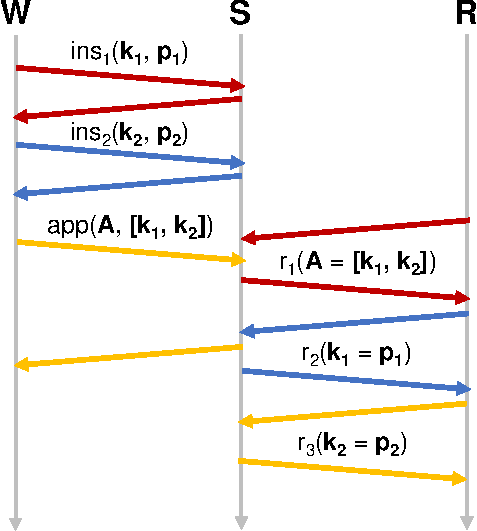
\includegraphics[scale=.45,page=1]{figs/motivation_figs.pdf}
  \label{fig:motivation:sdl}
}
\hfill
\subfloat[Naive \Multidispatch{}]{
  \includegraphics[scale=.45,page=2]{figs/motivation_figs.pdf}
  \label{fig:motivation:naive}
}
\caption{
A comparison of our example application when used with a
\singledispatch{} linearizable key-value store and a naive
attempt to introduce \multidispatch{}.
}
\label{fig:motivation}
\end{figure}

This problem is illustrated in Figure~\ref{fig:motivation}. We
show a user $W$ uploading two photos to an album $A$. At the same time, a
second user $R$ attempts to view the album. On the left, we show the
resulting Web server interactions with a linearizable key-value server $S$.
Because the key-value store guarantees
linearizability~\cite{herlihy1990linearizability} and $W$ issues the
two inserts and append sequentially, then a photo's blob will
always exist in the store once its key is visible in an album.
Thus, $R$'s second and third reads will never return \texttt{null}.

On the right, we show what can happen if we naively try to issue multiple
operations concurrently while still using a linearizable key-value store.
The uploader $W$ can issue all three operations concurrently, and the
viewer $R$ can issue the latter two reads concurrently (after getting the keys
from the list returned by the first read). In both cases, we see that the
end-to-end application latency is lower.

But because the uploader issues the operations concurrently,
their effects may appear in either order, so a photo's key may appear in an 
album before its blob is readable. Thus, $R$'s second and third reads may now
return \texttt{null}. The application code to view an album would therefore
need to be fixed to handle this new case.

Although the fix for our example application is relatively straightforward,
reasoning about the system's behavior in such cases (and how it impacts application behavior)
can quickly become complex.
Fixing applications also forces programmers to consider the system's implementation,
diminishing the usefulness of the consistency model.

In the next section, we propose a new \multidispatch{} 
consistency model, \md{}-linearizability, to remedy this 
tension. \Multidispatch{} linearizability explicitly allows 
applications to issue operations concurrently.

% Consequently, it 
% enables applications to achieve lower end-to-end latency. Provided 
% programmers obey a set of rules when parallelizing their applications 
% (described in Section~\ref{sec:}), an application interacting with a 
% multi-issue linearizability system will behave identically to the 
% original application interacting with a linearizable system. Thus, 
% programmers can reap these performance benefits without fear of 
% breaking their applications.
